%\documentclass[a4paper,10pt]{article}
\documentclass[11pt, twocolumn]{article}
\usepackage[utf8x]{inputenc}
\usepackage{multirow}
\usepackage{indentfirst}
\usepackage{graphicx}
\usepackage{amsmath}
\usepackage[version=3]{mhchem}
\usepackage{siunitx}
\usepackage{float}
\usepackage{subfigure}
\usepackage{morefloats}
\usepackage{caption}
\usepackage[spanish,activeacute]{babel}
\usepackage[pdftex]{hyperref}	%tiene que ir último?

\hypersetup{colorlinks = true}

\graphicspath{{figures/}}

%opening
\title{Modelado mediante elementos finitos del comportamiento de la membrana celular ante la electroporación}
%\author{Mauricio Alfonso}
\author{Mauricio Alfonso - LSC, FCEyN, \\Alejandro Soba - CSC-CONICET, \\Guillermo Marshall - INFIP, CONICET}

\begin{document}

\newcommand{\h}{\ce{H^+}}
\newcommand{\oh}{\ce{OH^-}}
\newcommand{\na}{\ce{Na^+}}
\newcommand{\cl}{\ce{Cl^-}}
\newcommand{\kvm}{$\si{\kilo\volt\per\metre}$}
\newcommand{\usec}{$\si{\micro\second}$}

\maketitle

%TODO poner nombres de poster, dc, lsc, que es para la afa, etc

\begin{abstract}
	La electroporación celular consiste en la aplicación de pulsos eléctricos de corta duración y alto potencial a una célula con el objetivo de crear poros en su membrana, logrando así una permeabilización que permita el ingreso de drogas o iones. Se realizaron simulaciones de células individuales a las que se les aplican pulsos a través de electrodos. Las simulaciones tienen en cuenta los siguientes fenómenos físicos: el potencial eléctrico en el dominio, la creación de poros en la membrana y la evolución de sus radios y el transporte de cuatro especies iónicas diferentes. Para ello se usó el método de elementos finitos en dos dimensiones con coordenadas cilíndricas, asumiendo la célula como un sólido de revolución.
	
	%TODO poner keywords
\end{abstract}

\section{Introducción}
En este trabajo se realizan simulaciones para estudiar el efecto de la electroporación en una célula. La electroporación es un método utilizado en el tratamiento del cáncer, que tiene como objetivo permeabilizar la membrana celular aplicando pulsos cortos a través de electrodos, permitiendo así el ingreso con mayor facilidad de agentes terapéuticos. De esta manera es posible reducir las dosis necesarias, minimizando costos y efectos secundarios.

Las simulaciones tienen en cuenta el campo eléctrico producido por los electrodos, la generación de poros en la membrana celular y la variación en el radio de los mismos con la consiguiente permeabilización de la membrana, y el transporte de cuatro especies iónicas: el ión hidrógeno (\h), el hidróxido (\oh), el catión sodio (\na) y cloruro (\cl), producto del potencial eléctrico.

Se implementó en \texttt{C++} usando el método de elementos finitos, y para reducir el costo computacional se aprovechó que la célula (asumida esférica) es un sólido de revolución, permitiendo así el uso de coordenadas cilíndricas en dos dimensiones. A diferencia de otros trabajos anteriores, los electrodos que generan el pulso eléctrico están dentro del dominio.

\subsection{Potencial eléctrico}
El potencial eléctrico es generado por dos electrodos con una diferencia de potencial constante durante la duración del pulso. Para el cálculo del potencial eléctrico en cada punto del dominio se utiliza la ecuación: 

\begin{equation} \label{eq:poisson}
	\nabla \sigma_{elem} \cdot (\nabla \phi) = 0 
\end{equation}

donde $\phi$ representa el potencial eléctrico y $\sigma_{elem}$ la conductividad del material \cite[p.~88]{fem-electro}.\\

Como consecuencia del potencial eléctrico se genera una diferencia de potencial entre el exterior e interior de la membrana celular, llamado potencial transmembrana (ITV). Se tiene en cuenta además que la membrana se carga como un capacitor en paralelo con una resistencia, por lo tanto el ITV crece según la ecuación:


\begin{equation} \label{eq:capacit} \begin{split}
	V_m = V_p\, (1 - e^{-t/\tau}) , \\ \textrm{con } \tau = \alpha\, C_m \left( \frac{1}{\sigma_i} + \frac{1}{2 \sigma_o} \right)
\end{split} \end{equation}

donde $ITV$ es el potencial transmembrana en un punto de la superficie de la célula, $V_p$ es el potencial obtenido por la ecuación \eqref{eq:poisson}, $t$ es el tiempo transcurrido desde el comienzo del pulso eléctrico, $\alpha$ es el radio de la célula, $C_m$ es la capacitancia superficial de la célula y $\sigma_i$ y $\sigma_o$ las conductancias intra y extracelulares respectivamente \cite{krass}.\\


\subsection{Generación de poros}
El potencial transmembrana genera poros hidrofílicos en la membrana. La densidad de estos poros se calcula con la ecuación:

\begin{equation} \label{eq:poros-crea}
	\frac{\partial N}{\partial t} = \alpha_c e^{(ITV/V_{ep})^2} \left( 1 - \frac{N}{N_0 e^{q \left(ITV/V_{ep} \right) ^2}} \right)
\end{equation}

donde $N$ es la densidad de poros en un determinado tiempo y posición de la membrana celular, $\alpha_c$ es el coeficiente de creación de poros, $ITV$ es el potencial transmembrana, $V_{ep}$ es el voltaje característico de electroporación, $N_0$ es la densidad de poros en equilibrio (cuando $ITV = 0$) y $q$ es una constante igual a $(r_m / r*)^2$, donde $r_m$ es el radio de mínima energía para $ITV = 0$ y $r*$ es el radio mínimo de los poros \cite{krass}.\\

Dado que el ITV es diferente en distintas regiones de la superficie celular, también lo es la densidad de poros generados.

\subsection{Radio de los poros}
Los poros generados según la ecuación \eqref{eq:poros-crea} tienen un radio inicial $r*$ igual a 0.51 $\si{\nano\metre}$. Este radio no permanece constante sino que varía en el tiempo y depende del ITV y del resto de los poros en la célula. Para cada poro individual su radio se calcula según la ecuación:

\begin{equation} \label{eq:poros-radio}
	\frac{\partial r}{\partial t} = \frac{D}{kT} \left( \frac{ITV^2 F_{max}}{1+r_h / (r+r_a)} + \frac{4 \beta}{r} \left(\frac{r_*}{r}\right)^4 - 2 \pi \gamma + 2 \pi \sigma_{\textrm{\tiny eff}} r\right)
\end{equation}

donde $r$ es el radio del poro, $D$ es el coeficiente de difusión para los poros, $k$ es la constante de Boltzmann, $T$ la temperatura absoluta, $ITV$ el potencial transmembrana, $F_{max}$ la máxima fuerza eléctrica para $ITV$ de 1V, $r_h$ y $r_a$ son constantes usadas para la velocidad de advección, $\beta$ es la energía de repulsión estérica, $\gamma$ es la energía del perímetro de los poros, y $\sigma_{\textrm{\tiny eff}}$ es la tensión efectiva de la membrana, calculada como

\begin{equation}
	\sigma_{\textrm{\tiny eff}} = 2 \sigma^\prime - \frac{2 \sigma^\prime - \sigma_0}{(1 - A_p / A)^2}
\end{equation}

donde $\sigma^\prime$ es la tensión de la interfase hidrocarburo-agua, $\sigma_0$ es la tensión de la bicapa sin poros, $A_p$ es la suma de las áreas de todos los poros en la célula, y $A$ es el área de la célula \cite{krass}. En la ecuación \ref{eq:poros-radio}, el primer término corresponde a la fuerza eléctrica inducida por el potencial transmembrana, el segundo a la repulsión estérica, el tercero a la tensión de línea que actúa en el perímetro del poro y el cuarto a la tensión superficial de la célula.\\

%esto último se puede borrar si no alcanza el espacio

\subsection{Transporte de especies}
Se calculan las concentraciones de cuatro especies iónicas: el ión hidrógeno (\h), el hidróxido (\oh), el catión sodio (\na) y el cloruro (\cl). Para ello se tiene en cuenta la difusión producto de las diferencias de concentración y la migración producto del campo eléctrico. Se utiliza la ecuación de conservación de masa de Nernst-Planck:

\begin{equation} \label{eq:trans}
	\frac{\partial C_i}{\partial t} = \nabla \cdot \left( D_i \nabla C_i + D_i z_i \frac{F}{R T} C_i \nabla \phi \right)
\end{equation}

donde $C_i$, $D_i$ y $z_i$ representan la concentración, el coeficiente de difusión y la valencia 
respectivamente de la especie $i$, para $i = $ \h, \oh, \na ó \cl.
$F$ es la constante de Faraday, $R$ la constante de los gases y $T$ la temperatura \cite{fodava}.\\

\subsection{Acoplamiento}
La permeabilización obtenida por los poros en una region de la membrana se puede expresar como un coeficiente que indica qué porción de la superficie celular está ocupada por los poros. Se actualizan los valores de conductividad y difusión de la membrana como un promedio pesado entre los valores originales y los del líquido que llena los poros, usando dicho coeficiente.

\section{Implementación}
Las simulaciones se realizaron con el método de elementos finitos sobre un dominio de coordenadas cilíndricas. Se generaron mallas bidimensionales con elementos cuadrilaterales usando el programa AutoMesh-2D \cite{automesh}. La mallas utilizadas tienen tres regiones: el líquido extra-celular, el citoplasma y la membrana celular. A diferencia de otros trabajos en los que no se modeló la membrana celular por ser extremadamente fina respecto del resto de la célula o se la modeló con un ancho superior al real, en este trabajo se modeló la membrana con su ancho real de 5 \si{\nano\metre}. Se generaron varias mallas, para células de tamaños entre 10 \si{\micro\metre} y 50 \si{\micro\metre}.\\

Los elementos que forman la malla tienen tamaño variable, siendo los cercanos a la membrana los de menor tamaño por ser la región de mayor interés. El intervalo temporal también es variable, siendo muy pequeño en los primeros microsegundos del pulso y aumentando con el paso del tiempo. A su vez las ecuaciones \eqref{eq:poros-crea} y \eqref{eq:poros-radio} corren con un intervalo temporal muy pequeño mientras que la ecuación \eqref{eq:poisson} tiene un intervalo más grande y la ecuación \eqref{eq:trans} uno aún más grande, por ser los cambios en las concentraciones de especies y el campo eléctrico mucho más lentos que los cambios en los poros de la membrana. \\

Para la ecuaciones \ref{eq:poisson} y \ref{eq:trans} se usaron condiciones de borde de Dirichlet con valores fijos en los bordes ocupados por los electrodos y Neumann en los otros bordes.\\

Con todo esto se realizaron varias simulaciones con células de radios entre 10 y 50 $\si{\micro\metre}$ y pulsos de 20 $\si{\milli\second}$ con potenciales entre 40 y 200 $\si{\kilo\volt\per\metre}$.

%TODO podría ir una imagen de la malla

\section{Resultados}
Se prestó especial atención al potencial transmembrana (ITV) obtenido en diferentes partes de la célula por ser el fenómeno que genera los poros. Se observó en todos los casos que en los primeros microsegundos del pulso el ITV aumenta debido a la capacitancia de la membrana. Una vez alcanzado un valor ligeramente superior a 1V el ITV comienza a disminuir hasta alcanzar un valor de equilibrio. Esto se debe a que los valores altos de tensión alcanzados crearon muchos poros en la membrana, disminuyendo así la conductividad de la misma y provocando una disminución en su caída de tensión. Los valores de ITV no son constantes en toda la célula, sino que son muy variables y dependen del ángulo polar $\theta$: en las regiones polares se alcanzan valores de ITV altos muy rápidamente, mientras que en las regiones cercanas al ecuador de la célula el ITV prácticamente no deja de ser 0 durante toda la simulación.

\begin{center}
	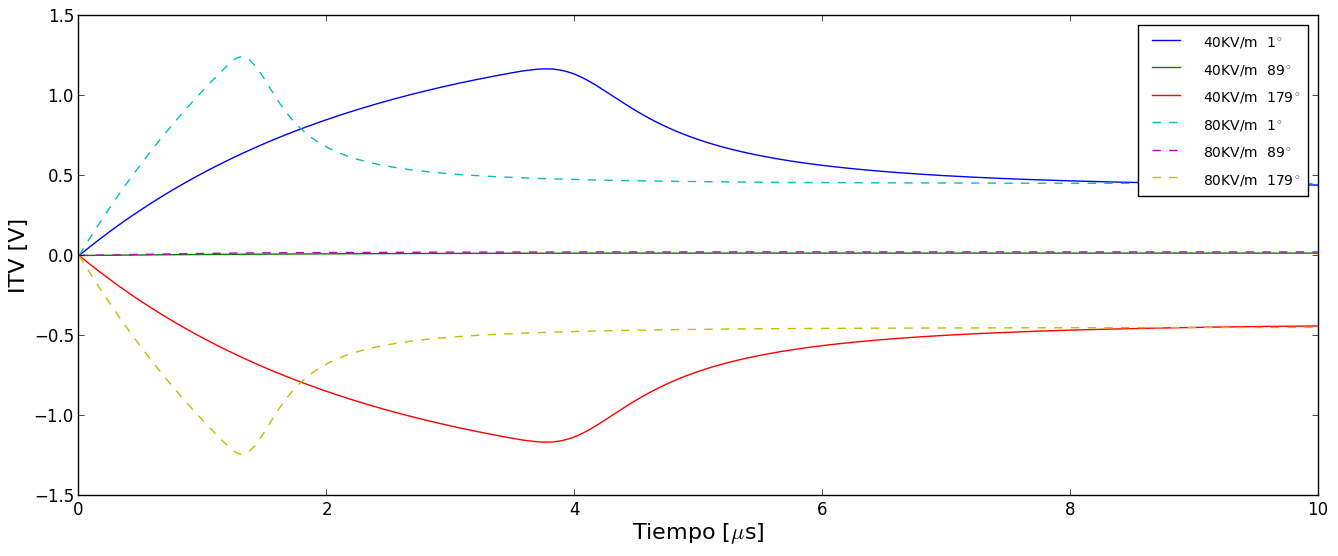
\includegraphics[width=1\linewidth]{itv-long}
	\captionof{figure}{ITV en función del tiempo para dos potenciales diferentes y diferentes ángulos polares.}
\end{center}

Experimentando con diferentes potenciales en los electrodos, se observó que superado un cierto umbral, un mayor potencial no aumenta el ITV, pero acelera el tiempo en el que se crean los poros y se alcanza el pico de tensión, que luego disminuye.

Se observó que el ITV alcanzado es suficiente para crear muchos poros en la membrana, pero la mayoría se sellan rápidamente, teniendo un radio considerable por un periodo muy corto de tiempo: a los 5 ms del pulso en todos los casos la cantidad de poros es mucho menor en instantes anteriores, aunque los pocos poros grandes que siguen existiendo parecen tener mayor radio que la mayoría de los poros en los instantes anteriores. La corta vida de la mayoría de los poros parece deberse a que la alta densidad de los primeros instantes reduce significativamente la conductancia de la membrana, y por lo tanto el ITV necesario para mantener los poros abiertos.

\begin{center}
	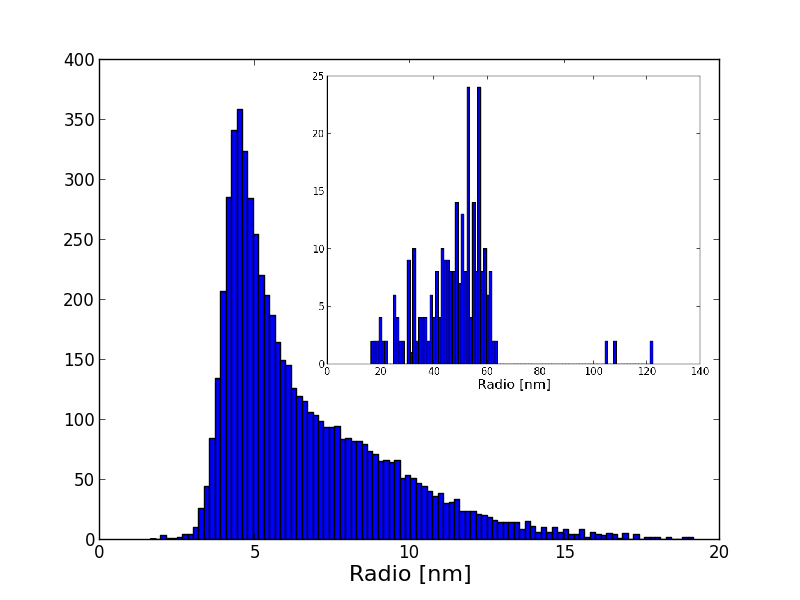
\includegraphics[width=1\linewidth]{hist-pip}
	\captionof{figure}{Distribución de radios de poros grandes (mayores a 1 \si{\nano\metre}) para una misma simulación en t = 5 \si{\micro\metre} y 5 \si{\milli\second}.}
\end{center}


En cuanto al transporte de especies, se observó que las especies \h y \oh ingresan con mucha facilidad al interior de la célula, siendo el \h la especie que más fácilmente ingresa. Por otra parte el \na y \cl ingresan en cantidades mucho menores, al menos para un solo pulso. El potencial aplicado por los electrodos parece influir positivamente en las concentraciones finales de las especies en el interior de la célula, excepto en las concentraciones de \cl, que no parecen aumentar al subir el potencial, e incluso disminuyen en algunas regiones interiores.

\begin{center}
	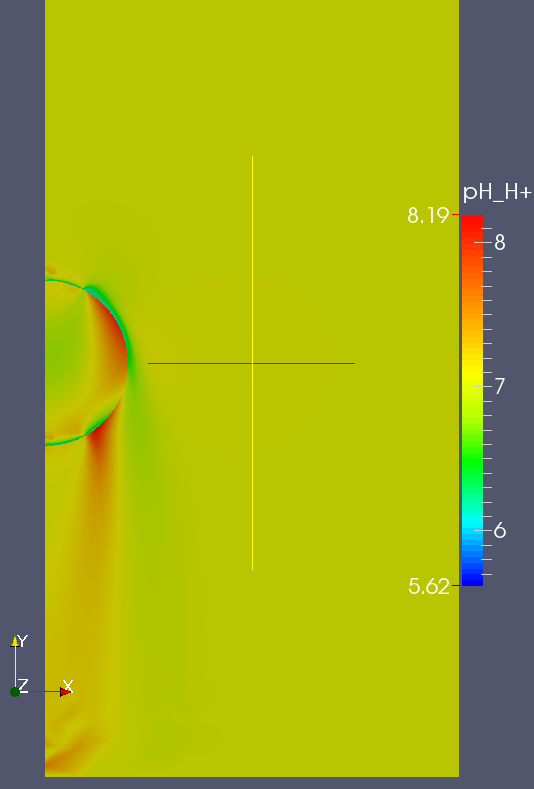
\includegraphics[width=0.52\linewidth]{H-ejemplo}
	\captionof{figure}{Concentración final de \h en el dominio para una célula de 10 \si{\micro\metre} de radio.}
\end{center}


\section{Conclusiones}

\begin{itemize}
	\item Más allá de un cierto umbral, no es posible aumentar el potencial transmembrana (ITV) aumentando la diferencia de potencial en los electrodos, ya que un mayor campo eléctrico sólo acelera el proceso de creación de poros, los que disminuyen la conductividad de la membrana, pero no aumenta el pico de tensión máximo alcanzado en el ITV.
	\item La mayoría de los poros creados se sellan muy rápidamente, antes de que lleguen las especies estudiadas a la membrana, y por lo tanto no sirven para permitir su ingreso.
	\item Un alto porcentaje de los poros creados se cierran durante el primer milisegundo, por lo que si se pretende permeabilizar la membrana para las especies estudiadas, se vuelve esencial repetir el pulso periódicamente. Queda pendiente para trabajos futuros estudiar varios pulsos periódicos y como la frecuencia y duración de los mismos afectan el transporte de especies al interior de la célula. 
\end{itemize}




\begin{thebibliography}{9}
%TODO meter las refs que faltan (ver preinforme)

\bibitem{puchiar}
	G. Puchiar, T. Kotnik, B. Valič and D. Miklavčič
	\emph{Numerical Determination of Transmembrane Voltage Induced on Irregularly Shaped Cells}
	Annals of Biomedical Engineering
	April 2006, Volume 34, Issue 4, Pages 642-652

\bibitem{fodava}
	Qiong Zheng, Duan Chen and Guo-Wei Wei
	\emph{Second-order Poisson Nernst-Planck solver for ion channel transport}
	Journal of Computational Physics
	Volume 230, Issue 13, 10 June 2011, Pages 5239–5262

\bibitem{krass}
	Wanda Krassowska and Petar D. Filev
	\emph{Modeling Electroporation in a Single Cell}
	Biophysical Journal
	Volume 92, Issue 2, 15 January 2007, Pages 404–417

\bibitem{fem-electro}
	Stanley Humphries, Jr.
	\emph{Finite-element Methods for Electromagnetics}
	2010

\bibitem{fem}
	O.C. Zienkiewicz and R.L. Taylor
	\emph{The Finite Element Method Volume I: The Basis}
	Butterworth-Heinemann,
	5th edition,
	2000

\bibitem{marino}
	Matías Daniel Marino, Dr. Pablo Turjanski, Dr. Nahuel Olaiz
	\emph{Electroporación en el tratamiento de tumores: modelos teóricos y experimentales}
	2013

\bibitem{automesh}
	\href{http://www.automesh2d.com/}{http://www.automesh2d.com/}

\end{thebibliography}

\end{document}
